%%%%%%%%%%%%%%%%%%%%%%%%%%%%%%%%%%%%%%%%%
% Journal Article
% LaTeX Template
% Version 1.3 (9/9/13)
%
% This template has been downloaded from:
% http://www.LaTeXTemplates.com
%
% Original author:
% Frits Wenneker (http://www.howtotex.com)
%
% License:
% CC BY-NC-SA 3.0 (http://creativecommons.org/licenses/by-nc-sa/3.0/)
%
%%%%%%%%%%%%%%%%%%%%%%%%%%%%%%%%%%%%%%%%%

%----------------------------------------------------------------------------------------
%	PACKAGES AND OTHER DOCUMENT CONFIGURATIONS
%----------------------------------------------------------------------------------------

\documentclass[11pt]{article}

\usepackage[sc]{mathpazo} % Use the Palatino font
\usepackage[utf8]{inputenc}
\usepackage[T1]{fontenc} % Use 8-bit encoding that has 256 glyphs
\linespread{1.05} % Line spacing - Palatino needs more space between lines
\usepackage{microtype} % Slightly tweak font spacing for aesthetics

%\usepackage[hmarginratio=1:1,top=32mm]{geometry} % Document margins
%\usepackage{multicol} % Used for the two-column layout of the document
\usepackage[hang, small,labelfont=bf,up,textfont=it,up]{caption} % Custom captions under/above floats in tables or figures
\usepackage{booktabs} % Horizontal rules in tables
\usepackage{float} % Required for tables and figures in the multi-column environment - they need to be placed in specific locations with the [H] (e.g. \begin{table}[H])
\usepackage[hidelinks]{hyperref} % For hyperlinks in the PDF

\usepackage{lettrine} % The lettrine is the first enlarged letter at the beginning of the text
%\usepackage{paralist} % Used for the compactitem environment which makes bullet points with less space between them

\usepackage{todonotes}
\usepackage{graphicx}
\usepackage{amsmath,amssymb,amsfonts}
\usepackage{subcaption}
\providecommand{\abs}[1]{\left \lvert #1 \right \rvert}

\usepackage{abstract} % Allows abstract customization
\renewcommand{\abstractnamefont}{\normalfont\bfseries} % Set the "Abstract" text to bold
\renewcommand{\abstracttextfont}{\normalfont\small\itshape} % Set the abstract itself to small italic text

\usepackage{titlesec} % Allows customization of titles
\renewcommand\thesection{\Roman{section}} % Roman numerals for the sections
\renewcommand\thesubsection{\Roman{subsection}} % Roman numerals for subsections
\titleformat{\section}[block]{\large\scshape\centering}{\thesection.}{1em}{} % Change the look of the section titles
\titleformat{\subsection}[block]{\large}{\thesubsection.}{1em}{} % Change the look of the section titles

\usepackage{fancyhdr} % Headers and footers
\pagestyle{fancy} % All pages have headers and footers
\fancyhead{} % Blank out the default header
\fancyfoot{} % Blank out the default footer
%\fancyhead[C]{Running title $\bullet$ November 2012 $\bullet$ Vol. XXI, No. 1} % Custom header text
\fancyfoot[RO,LE]{\thepage} % Custom footer text

%----------------------------------------------------------------------------------------
%	TITLE SECTION
%----------------------------------------------------------------------------------------

\title{\vspace{-15mm}\fontsize{24pt}{10pt}\selectfont\textbf{Local Adaptive
Optimization of Time Step}} % Article title

\author{
\large
\textsc{Malte Stær Nissen}\thanks{Thanks to my supervisor Sune Darkner for
helping me realize this project}\\[2mm] % Your name
\normalsize University of Copenhagen \\ % Your institution
\normalsize \href{mailto:nissen@diku.dk}{nissen@diku.dk} % Your email address
\vspace{-5mm}
}
\date{}

%----------------------------------------------------------------------------------------

\begin{document}

\maketitle % Insert title

\thispagestyle{fancy} % All pages have headers and footers

%----------------------------------------------------------------------------------------
%	ABSTRACT
%----------------------------------------------------------------------------------------

%\begin{abstract}


%\end{abstract}

%----------------------------------------------------------------------------------------
%	ARTICLE CONTENTS
%----------------------------------------------------------------------------------------

%\begin{multicols}{2} % Two-column layout throughout the main article text

\section{Introduction}
\lettrine[nindent=0em,lines=3]{S} imulations of large hyperelastic materials
such as brain tissue
can be very time consuming. When working with materials of varying density
of vertices/scale of mesh, the highest densities often give the most
strict bounds on size of the timestep of the simulation in order to keep
the materials (and grids) stable and the discretization correct.

In a ``standard'' simulation with a global timestep size we need to compute
possibly unnecessarily many computations on the coarser parts of the material
caused by this bound. When furthermore having materials with a large amount
of somewhat equally distributed vertices and smaller patches of detailed
areas with higher density of vertices, it would be an advantage to be able
to perform large timesteps for the majority of the material (the coarse
parts) and smaller steps for the local patches where vertices could cause
instability. We call the concept of varying the timestep local adaptive
optimization of timestep (LAOT), in which ``local'' either refers to spatial
locality (as described above) or time locality where the timestep is global
for all vertices but varies during the simulation.

We will in this report
study possible approaches for application of LAOT. In order to keep the focus
on possible LAOT methods and remove unneccessary complexities, we will study
the simple 1 dimensional simulation of a mass-spring system and try to apply
LAOT for it. Afterwards we will shortly discuss the application of our gained
knowledge to the domain of hyperelastic material simulation and simulations in
general.

%------------------------------------------------

\section{Previous work} According to \cite{Gander:2013} local timestepping
was first studied in the community of ordinary differential equations (ODE)
with Rice \cite{rice:1960} developing the split Runge-Kutta methods (multi
rate Runge-Kutta methods). The concept behind these methods is the splitting
of the ODEs into multiple (two components in \cite{rice:1960}) components of
which each component needs to be integrated in different scales. A strategy
is chosen as proposed in \cite{Kvaernoe:1999} of either computing the coarser
part first (``Fastest first strategy'') followed by the finer part or vice
versa (``Slowest first strategy''). In order to perform these sequential
computations either interpolation or extrapolation of the first computation
is performed to compute the second part in each timestep. The different
timestep sizes can be adapted to fit the model in each step as well. See
\cite{Kvaernoe:1999} and \cite{Gear:1984} (similar strategy for linear multi
step methods) for more detailed descriptions of the two strategies.

In the partial differential equations (PDE) community, the adaptive time
stepping area was explored and developed with the goal of simulating
very specific known problems such as the (hyperbolic) wave equations
and (parabolic) heat equations instead of more general applications. We
will refrain from describing the methods further in this report, but a
short description and comparison of the specific methods can be found in
\cite{Gander:2013}. Generally the methods developed at first all make use
of the same basic concepts for making the local adaptive timestepping:
Interpolation, extrapolation, prediction and correction, which we are going to
use in the work of this report as well.

Recently newer and faster methods with local timestepping have been developed
on the basis of nonlinear PDEs and the work performed in this field in
the 80s and 90s. First the multi resolution (MR) schemes for creating
space-adaptive discretizations and refinements of these were developed, see
\cite{Berger:1984}. Then multiple MR based schemes were developed. Domingues
et al. \cite{Domingues:2008} is one of the more recent of these MR schemes.
They describe a local scale-dependent timestepping for a space-adaptive multi
resolution scheme using the finite volume method in order to obtain speed-up
using larger time-steps without violating a defined stability constraints,
which is essentially the same motivation as this report. The method is based
on an explicit Runge-Kutta method of second order. As expected the timestep
size is imposed by a stability condition of the explicit Runge-Kutta on the
finest scale, which increases with the scale of the mesh and hence we are able
to increase the timestep as well without violating the stability condition.


%------------------------------------------------

\section{Methods}
\label{sec:methods}

With no prerequisites within the field of mass simulations we will first
consider the 1D problem of simulating a mass-spring system using the explicit
(forward) Euler method.

Second we will propose and test out three different methods for applying LAOT
to the simulation.

Third and last we will discussion the results and how we could apply our
knowledge of LAOT for hyperelastic material.

\subsection{1D mass-spring system} Mass-spring systems are systems simulating
a set of vertices interconnected by springs in various ways to obtain
desirable physical properties. The motion of the springs and vertices are
then simulated as a function of the time elapsed. Examples of application of
mass-spring systems are simulation of cloth or hair. When performing simulations
we want to avoid a switch of position of spring-connected vertices caused by the
timestep size of the simulation, since this invalidates our discretization of
the domain. Furthermore we want to perform as few timesteps as possible in order
to get to the final simulation state by using as big timesteps as possible
without affecting the outcome of the simulation.

When simulating the mass-spring system we perform the following steps:
\begin{enumerate} \item Initialize system \item Calculate forces \item
Calculate derrivatives \item Update positions and velocities \item Update time
\item Go to step 2 if the simulation has not reached it's maximum simulation
time. \end{enumerate} We now describe the details of each of the steps of
the simulation.

Our 1D mass-spring system consists of a set $V$ of vertices and a set
$S$ of springs. Each vertex $v \in V$ has a specified position $p_v$,
mass $m_v$, force $F_v$ and velocity $u_v$, and each spring $s \in S$
has two endpoints vertices $p_{f,s} \in V$ and $p_{t,s} \in V \setminus
p_{f,s}$, a damping factor $d_s$, a stiffness constant $K_s$ and a rest length
$l_{0,s}$. All these variables and constants combined describe the state
of the mass-spring system at each time $t$ during a simulation. All these
variables are initialized in step 1.

The total force of a spring is the sum of the spring force $F_{h,d}$
calculated by using Hooke's Law (see \cite[p.~439]{Young:2010})
and the damping force $F_{C,d}$ using a simple damping method (see
\cite[p.~457]{Young:2010}): \begin{align} \nonumber l_d &= p_{l,d} -
p_{r,d} \\ \label{eq:hooke} F_{h,d} &= -k_d x_d = -k_d (l_d - l_{0,d}) \\
\label{eq:damping} F_{C,d} &= -C_d \frac{\partial x_d}{ \partial t} = - C_d
\frac{\left(v_{l,d} - v_{r,d}\right) l_d}{\abs{l_d}} \\ F_d &= F_{h,d} +
F_{C,d} \end{align} \todo{Maybe add direction correction: $F_d \cdot (-l_d
/ \abs{l_d})$} in which $p_{l,d}$ and $p_{r,d}$ are the positions of the
left and right endpoints of the spring $d$ respectively, and $v_{l,d}$ and
$v_{r,d}$ are the velocities of the left and right endpoint vertices of the
spring $d$ respectively, and $F_d$ is the total force of spring $d$.

When calculating the forces applied by each spring, we add the total spring
force $F_d$ to the left endpoint of the spring and subtract $F_d$ from the
right endpoint since both endpoints are affected equally in opposite direction
by the spring $d$ connecting them. These spring forces are calculated in step
2 of the simulation.

We now know how to calculate the force of the spring system and apply it to
the vertices. In order to calculate the derrivatives of the system (step 3) we
use Newton's second law of motion (see \cite[p.~112-115]{Young:2010}) to get
the difference in speed $\Delta u_v$ and position $\Delta p_v$ of each vertex
$v$ using a given timestep size $\Delta t$: \begin{align} \label{eq:delta_u}
\Delta u_v &= \frac{\partial u_v}{\partial t} \Delta t = \frac{F_v}{m_v}
\Delta t \\ \label{eq:delta_p} \Delta p_v &= u \Delta t \end{align}

As mentioned in the beginning of this section we have chosen to use the
explicit Euler method defined below in equation \ref{eq:explicit_euler}
to calculate the time ``integration'' \cite{Flaherty} when stepping through
the simulation. Given a variable $x$ as a function of the time $t$, the
variable $x$ at the time $t + \Delta t$ is defined as: \begin{align}
\label{eq:explicit_euler} x(t+\Delta t) &= x(t) + \Delta t \frac{\partial
x(t)}{\partial t} \end{align} Applying this method for the timestepping
of our simulation we get the two following position and velocity update
equations using equations \ref{eq:delta_u} and \ref{eq:delta_p}: \begin{align}
p_v(t+\Delta t) &= p_v(t) + \Delta p_v \\ u_v(t+\Delta t) &= u_v(t) + \Delta
u_v \end{align} We use these equations to perform step 4 of the simulation.

Step 5 is a simple update of the time: $t = t + \Delta t$ and step 6 describes
itself.

We have now fully described the simple case of simulating a mass-spring system
using the explicit Euler method and the next subsections describe the three
different methods/modifications for applying LAOT to the simulation just
described. The three methods are using different ideas to implement LAOT. They
all include using some sort of heuristics in order to perform the adaption of
the methods. We developed and tested these heuristics as we developed the
methods (chronologically) and hence most of the heuristics could potentially be
used on all three methods and not only the methods on which they were used. In
case the methods are working succesfully, they could furthermore be combined to
generate ie. fully atomic timestepping (both time and spatial adaptive).

\subsection{Adapt-on-switch}
\label{sec:method_switch}
The first LAOT method we propose is time-adaptive. We perform a simulation
with an initial timestep size. In each step we try to predict whether a timestep
of the same size using the current velocities will result in a switch of the
left and right vertices of any of the springs. If this is the case, we should
try to avoid the switch by decreasing the timestep of the current iteration,
re-calculate the velocity and position changes and resume stepping of the
simulation using the new timestep size. When switches aren't detected anymore
we gradually increase the timestep of the simulation again. We call this
method the adapt-on-switch method.

The switch of two endspoints connected by a spring $d$ can easily be
calculated by checking the length ($p_{l,d} - p_{r,d}$) of the spring before
and after a position update. If the sign of the length differs, the two
points must have switched sides and hence adaption of the timestep should be
performed. The adaption of the timestep can either be done by division of the
current timestep by a constant or by having a finite set of timestep sizes to
choose from.

\subsection{Atomic Updating using Heuristics}
The second LAOT method we propose is space-adaptive. We perform simulations
using a fixed timestep size. In each iteration we perform position update of
all vertices, but only re-calculate acceleration and velocity of the springs
and points that fulfill some defined heuristics and hence the method is called
``Atomic Updating using Heuristics'' (AUH).

The heuristics can be chosen to fit the domain of the simulation, but we have
chosen to use the number of steps since last update, $n_{last}$, and the ratio
between the current spring length and the spring length at the last update
$r_{last}$. This should force a bound on the maximal number of timesteps
before update as well as force frequent updates when the spring is affected by a
high acceleration in opposite direction of the current velocity/direction of
change. \todo{Explain length ratio thought}. Further details are explained in
section \ref{sec:experiments_atomic}.

\subsection{Global Estimated Acceleration}
The third and last LAOT method we propose is time-adaptive. The simulations are
done using an initial timestep size and define the timestep of each iteration
based on a heuristic using the acceleration of the springs, and hence we call
the method Global Estimated Acceleration (GEA). We know that the force and hence
acceleration of a spring is somewhat linear close to the spring's rest length
and it ``bends'' off as the spring is streched or contracted further away from
the rest length. Based on this knowledge we will try to make a heuristic
telling us about the needed timestep size at any given point during the
simulation. The smallest needed timestep defines the global timestep for that
given step.

For this simple 1D example we use the inverse of the acceleration
for adapting the timestep and hence the heuristic is defined as:
\begin{align}
    \frac{1}{a} &= \frac{1}{\frac{-kx}{m}} = \frac{m}{-kx} \\
    \label{eq:inverse}
    \Delta t &= \text{min}\left( \frac{1}{\abs{a} + 0.1} \right )
\end{align}
We have added a small value (0.1) in order to avoid the timestep to increase
exponentially towards infinity as $\abs{a}$ approach 0. Furthermore a scaling
of the timestep could be needed depending on the scale of the simulation mesh.
Further details are explained in section \ref{sec:experiments}.

Our though is that for more
complex simulations we are able to make estimates of this type less costly than
performing the actual simulations of a small fixed size timestep.

%------------------------------------------------

\section{Experiments, results and discussion}
\label{sec:experiments}

We first give an example of the actual application of LAOT using the
standard simulation of mass spring particles. Figure \ref{fig:std} shows two
simulations of the same set of particles distributed with two different scales
simulated for 250 seconds each. All the springs $s \in S$ are initiated in a
stretched state/position with a length 1.25 times longer than the rest length,
damping and stiffness constants $C_s = 0.5, K_s = 0.5$, and all vertices $v
\in V$ have a mass of $m_v = 30$. Given this initial state all springs should
start constracting since they are in a stretched position and eventually
somewhere further in time stabilize at the rest position since we have added
the damping force to the system.

\ref{fig:std_multi_30fps} shows a simulation of the system described above
using 30 fps and Figure \ref{fig:std_multi_1fps} shows the simulation using 1
fps. We clearly see that using a timestep of 30 fps the simulation is stable
and able to handle the compression of all the small springs around $t = 110$
whereas a switch occurs when simulating at 1 fps. This switch causes ripples
of sideeffects for the rest of the simulation and hence the final result is
incorrect. No switches of the longer springs are however occuring and hence
these pose no problem at 1 fps. We will use this simulation for testing all
three LAOT methods proposed in section \ref{sec:methods}.

\begin{figure}[H]
    \begin{subfigure}[t]{0.5\textwidth}
        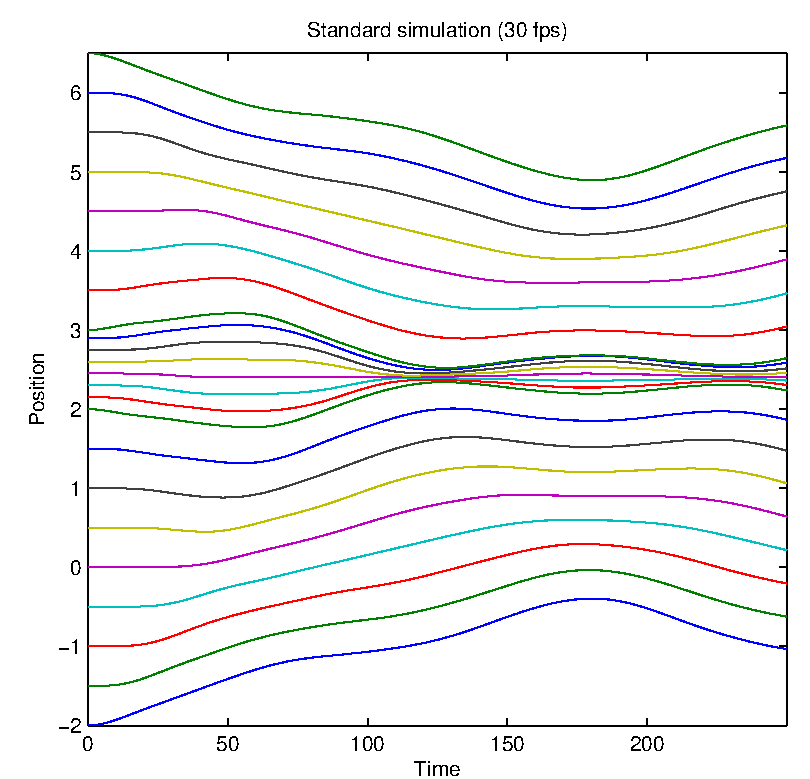
\includegraphics[width=\textwidth]{../images/standard_multiscale_30fps.pdf}
        \caption{30 fps}
        \label{fig:std_multi_30fps}
    \end{subfigure}
    \begin{subfigure}[t]{0.5\textwidth}
        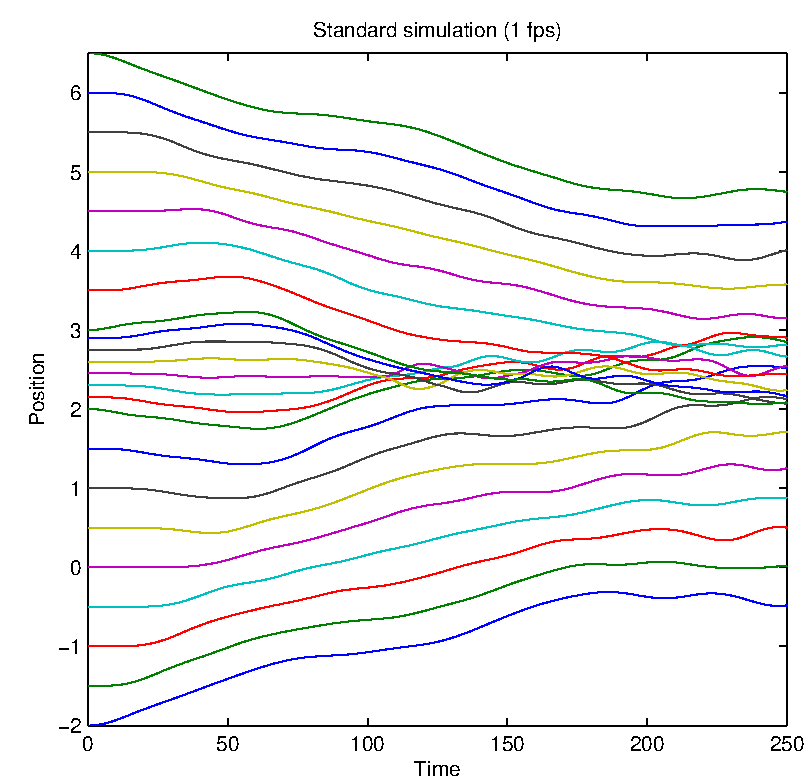
\includegraphics[width=\textwidth]{../images/standard_multiscale_1fps.pdf}
        \caption{1 fps}
        \label{fig:std_multi_1fps}
    \end{subfigure}
    \caption{Standard simulations of particles distributed with two scales using
    different timestep sizes}
    \label{fig:std}
\end{figure}

%\begin{figure}[H]
%    \begin{subfigure}[t]{0.5\textwidth}
%        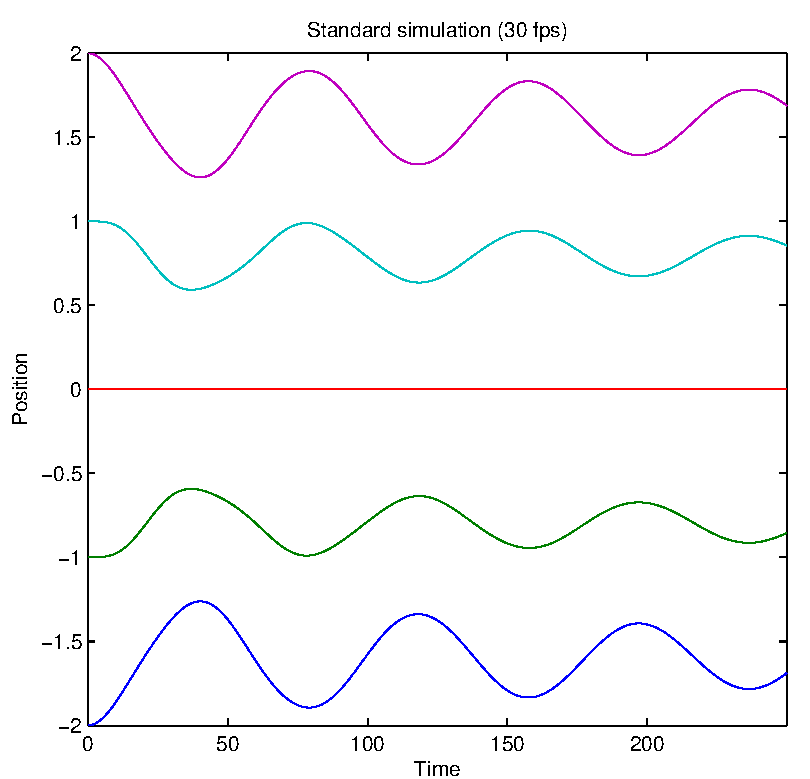
\includegraphics[width=\textwidth]{../images/standard_uniform_30fps.pdf}
%        \caption{30 fps}
%        \label{fig:std_uni_30fps}
%    \end{subfigure}
%    \begin{subfigure}[t]{0.5\textwidth}
%        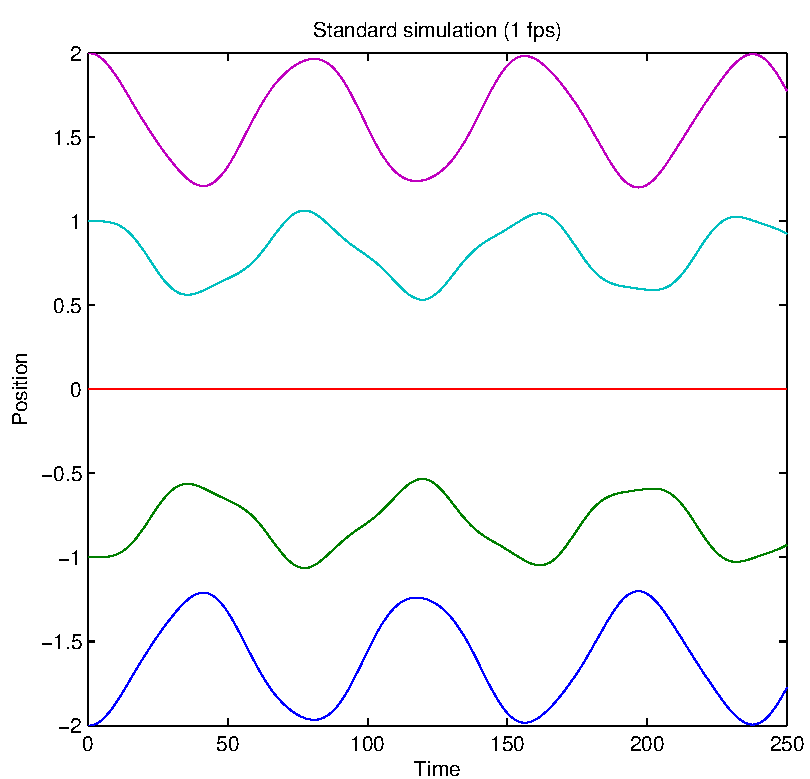
\includegraphics[width=\textwidth]{../images/standard_uniform_1fps.pdf}
%        \caption{1 fps}
%        \label{fig:std_uni_1fps}
%    \end{subfigure}
%    \caption{Standard simulations of particles distributed uniformly using
%    different timestep sizes}
%\end{figure}

\subsection{Adapt-on-switch}
As mentioned in section \ref{sec:method_switch} the adapt-on-switch method
can be implemented using either a relative or a absolute adaption of the
timestep. In our experiments we have tested out both methods defining the
relative adaption to scale the timestep by a factor of $\frac{1}{100}$ and
the absolute solution to set the timestep to $\frac{1}{30}$ when switches are
detected since this generated nice simulations for the standard simulation .
Furthermore the up-scaling for the relative scheme is set to a factor of 10
since we wish to avoid running into new switches immediately.

Figure \ref{fig:switch} shows the result of running simulations
described earlier at 1 fps using the adapt-on-switch scheme, where
the red crosses mark timesteps where a switch is predicted in the
following step and hence the schemes are ``activated''. Figure
\ref{fig:switch_multi_1fps_relative} is simulated using the relative scheme
and figure \ref{fig:switch_multi_1fps_absolute} is simulated using the
absolute scheme. As we clearly see in both figures the schemes fail to correct
the simulations in spite of the switch prediction. Once the first switch
occurs the simulation will change behavior and hence the first red cross marks
the point at which the simulation can be rejected from being correct.

After having made these observations we furthermore tested out a third way of
creating the scheme by predicting how long a timestep we could take before the
switch would occur and then divide this steplength by 2 to get a new timestep
length. This generated infeasibly small timesteps forcing us to stop the
simulation too early.

Taking these observations into account we can safely say that the
adapt-on-switch method/scheme is not working for our simulation. This does
however not mean that the method couldn't work for other domains or other
refinements of the method. The problem with the scheme is that the prediction
of switches is done too late in the simulation and hence once we detect
the switches it's too late to do anything about them given our model of
the mass-spring system. In order for the scheme to work properly it should
therefore be modified to be able to perform the detection of switches earlier
in the simulation.

In the real world the spring force would ``bend'' towards $\pm \infty$ once
the spring is stretched or contracted too much and hence the linear model that
we use doesn't suffice when using the adapt-on-switch scheme. Having used a
more realistic choice of model could possibly have had a positive impact of
the use of this scheme since this would cause the spring force of the spring
in question to grow in order to avoid the switch. \todo{Maybe the section
above should be moved to a discussion section.}

\begin{figure}[H]
    \begin{subfigure}[t]{0.5\textwidth}
        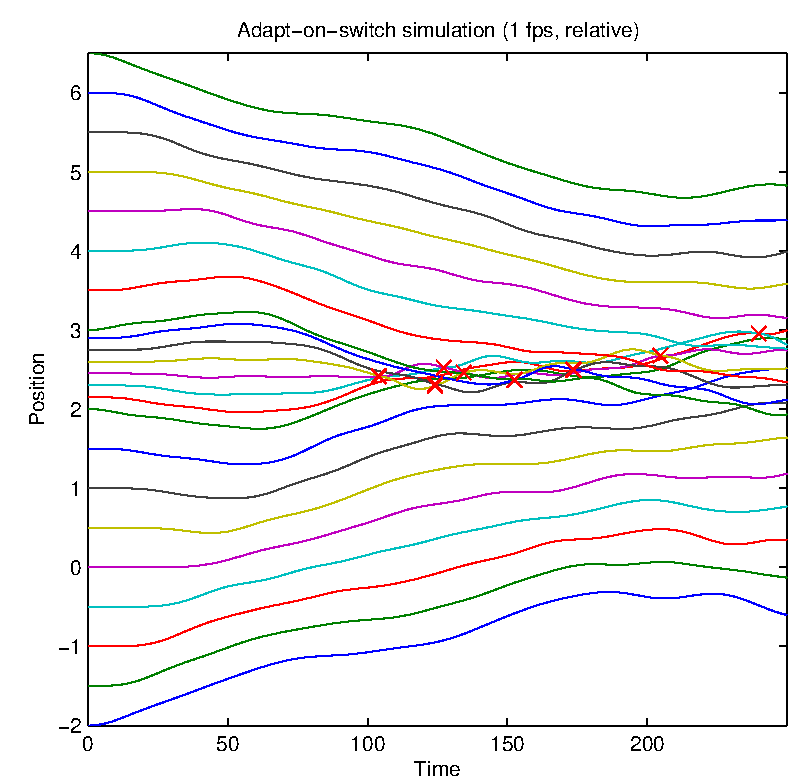
\includegraphics[width=\textwidth]{../images/switch_multiscale_1fps_relative.pdf}
        \caption{Relative timestepping ($\Delta t = \frac{\Delta t}{100}$)}
        \label{fig:switch_multi_1fps_relative}
    \end{subfigure}
    \begin{subfigure}[t]{0.5\textwidth}
        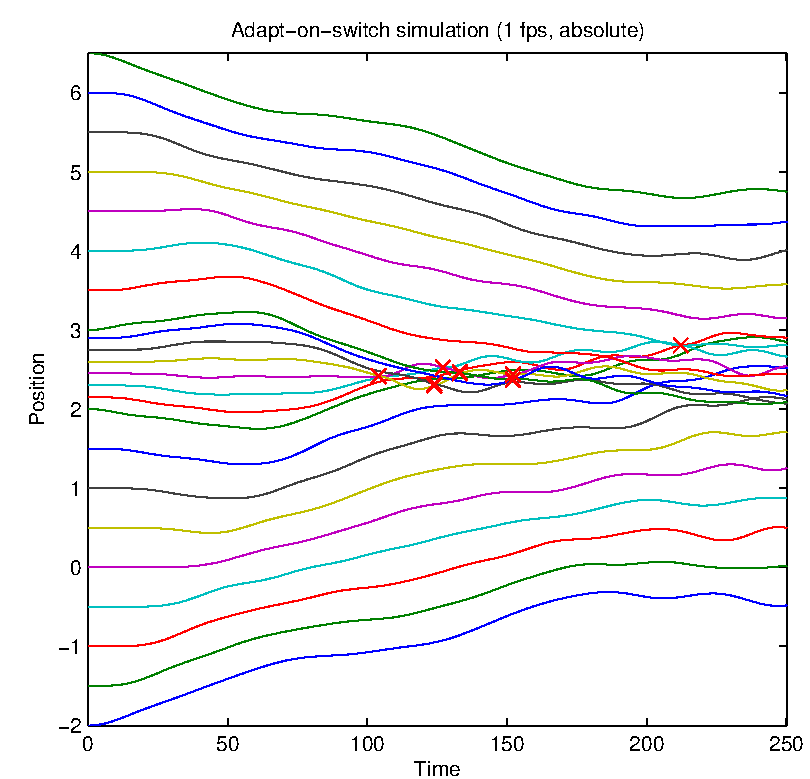
\includegraphics[width=\textwidth]{../images/switch_multiscale_1fps_absolute.pdf}
        \caption{Absolute timestepping ($\Delta t = \frac{1}{30}$)}
        \label{fig:switch_multi_1fps_absolute}
    \end{subfigure}
    \caption{Adapt-on-switch simulation of particles distributed with two
scales using 1 fps. The red crosses mark times at which the scheme predicts a
switch in the following iteration.}
    \label{fig:switch}
\end{figure}

\subsection{Atomic Updating using Heuristics}
\label{sec:experiments_atomic}
The AUH method concists of two heuristics for determining whether an element
should be updated or not: steps since last update $l_{last}$, and the ratio
between the spring length in last update and the current length $r_{last}$.

We first test the method using only the first heuristic which will give
us synchronized updates of all vertices every $r_{last}$ step. Using the
same setup as the standard simulation we perform simulations using the AUH
method with the length ratio heuristic ignored by setting the limit of
the ratio to infinity. We set the timestep to $\Delta t = \frac{1}{10}$
(10 fps) and vary $l_{last}$. Figure \ref{fig:atomic_multi_sbound} shows
the resulting simulations where figures \ref{fig:atomic_multi_10sbound},
\ref{fig:atomic_multi_68sbound}, and \ref{fig:atomic_multi_69sbound} uses
an $l_{last}$ of 10, 68, and 69 respectively.

Simulating using 10 fps and $l_{last} = 10$ gives us the same amount
of velocity updates as the standard simulation using 1 fps (which had
switches), but gives us a nice and smooth simulation with no problems.
As can be seen in the figures \ref{fig:atomic_multi_68sbound} and
\ref{fig:atomic_multi_69sbound} we are able to perform the simulation using
$l_{last} = 68$ without having switches occuring whereas using $l_{last} =
69$ results in switches occuring. In other words we are able to perform the
simulation at 10 fps but with 6.8 seconds between acceleration and velocity
calculations. This is a result of combining the explicit Euler method with
the AUH scheme since the scheme simply extrapolates the position at the last
acceleration and velocity update to a position close in time to the next
update position and then uses this position when updating the acceleration and
velocity again. Had we chosen an alternative time integration method this
advantage would most likely have been eliminated and let us perform the larger
timesteps with the standard simulation.

We now turn our attention towards the second heuristic.

\begin{figure}[H]
    \begin{subfigure}[t]{0.5\textwidth}
        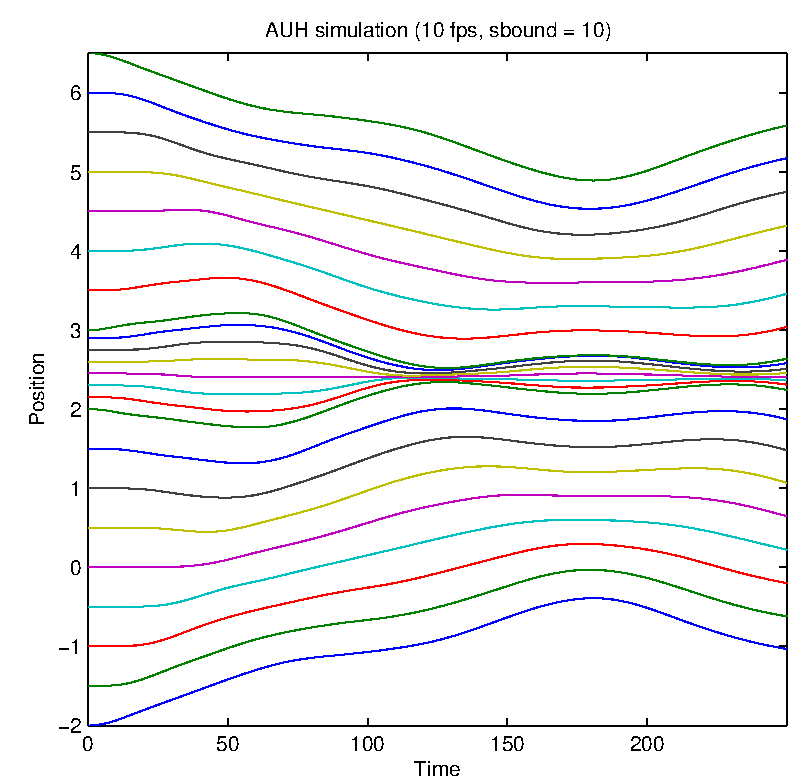
\includegraphics[width=\textwidth]{../images/atomic_multiscale_10fps_10sbound.pdf}
        \caption{$l_{last} = 10$, $r_{last}$ ignored}
        \label{fig:atomic_multi_10sbound}
    \end{subfigure}
    \begin{subfigure}[t]{0.5\textwidth}
        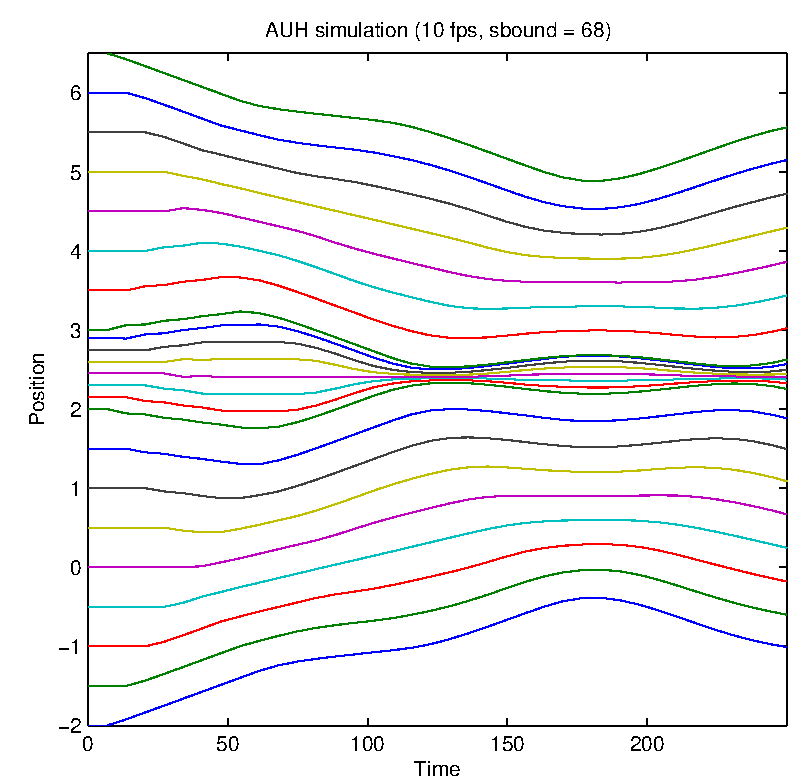
\includegraphics[width=\textwidth]{../images/atomic_multiscale_10fps_68sbound.pdf}
        \caption{$l_{last} = 68$, $r_{last}$ ignored}
        \label{fig:atomic_multi_68sbound}
    \end{subfigure}
    \begin{subfigure}[t]{0.5\textwidth}
        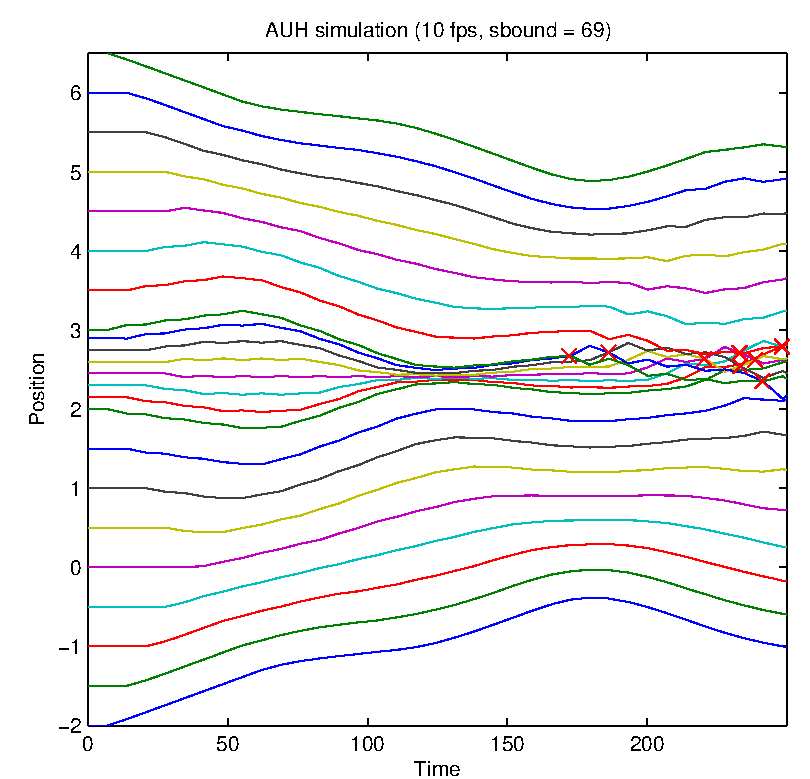
\includegraphics[width=\textwidth]{../images/atomic_multiscale_10fps_69sbound.pdf}
        \caption{$l_{last} = 69$, $r_{last}$ ignored}
        \label{fig:atomic_multi_69sbound}
    \end{subfigure}
    \begin{subfigure}[t]{0.5\textwidth}
        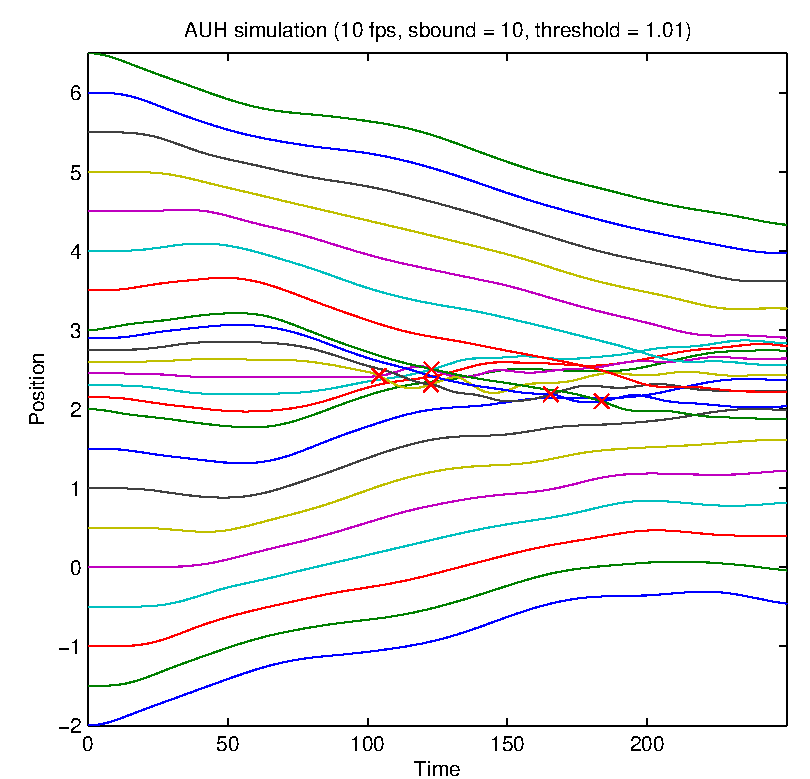
\includegraphics[width=\textwidth]{../images/atomic_multiscale_10fps_both.pdf}
        \caption{$l_{last} = 10, r_{last} = 1.01$}
        \label{fig:atomic_multi_both}
    \end{subfigure}
    \caption{Simulations using the AUH method at 10 fps with various number of
    steps since last update.}
    \label{fig:atomic_multi_sbound}
\end{figure}

\begin{figure}
    \begin{subfigure}[t]{0.5\textwidth}
        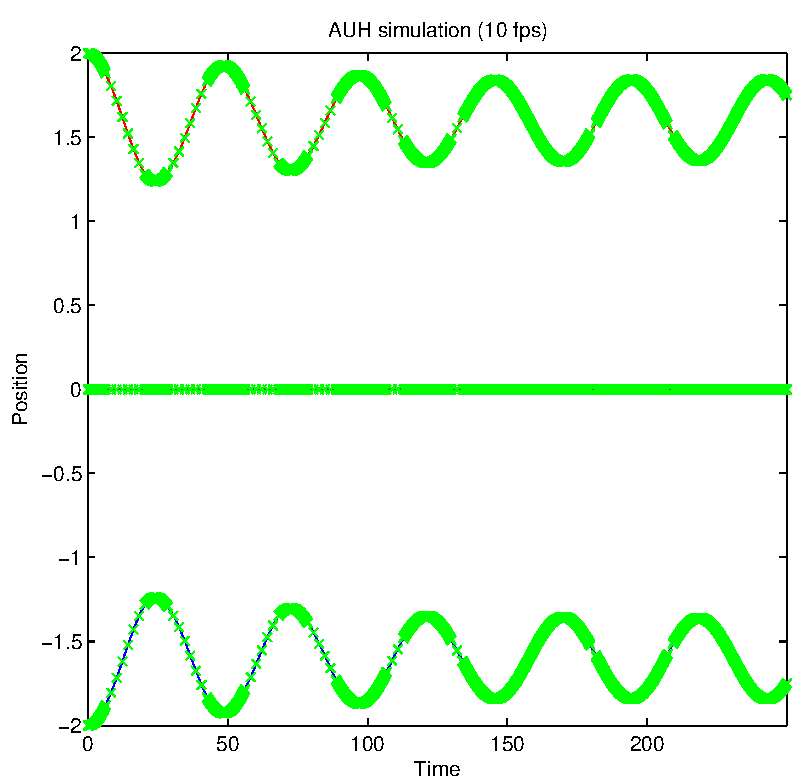
\includegraphics[width=\textwidth]{../images/atomic_uniform_10fps_0.pdf}
        \caption{}
        \label{fig:atomic_uniform_10fps_0}
    \end{subfigure}
    \begin{subfigure}[t]{0.5\textwidth}
        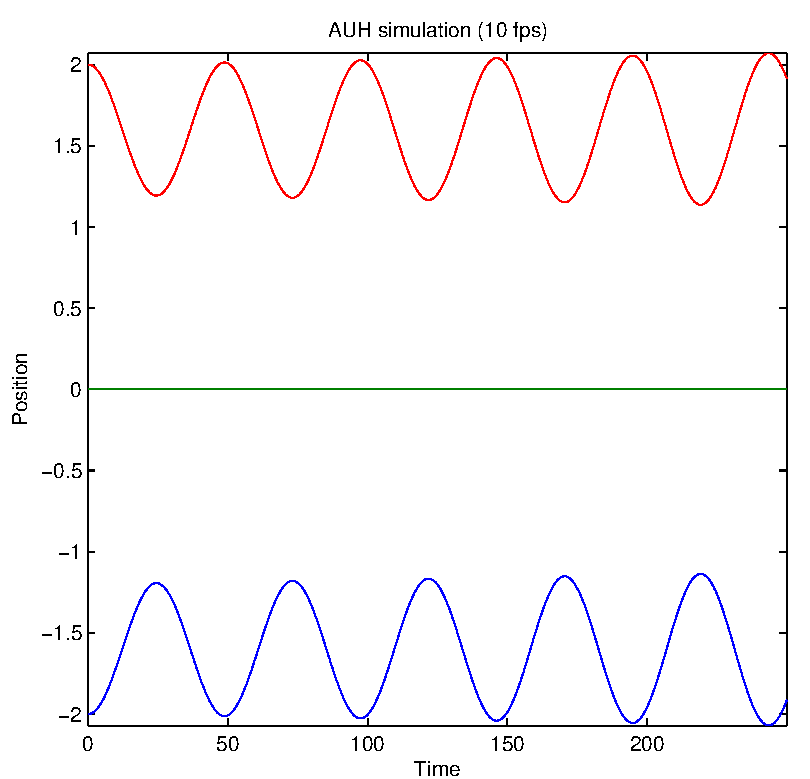
\includegraphics[width=\textwidth]{../images/atomic_uniform_10fps_1.pdf}
        \caption{}
        \label{fig:atomic_uniform_10fps_1}
    \end{subfigure}
    \caption{}
    \label{fig:atomic_uniform}
\end{figure}


if ratio then too much dampening caused by lack of updates: Example: Simple with
3 springs

\subsection{Global Estimated Acceleration}
In the GEA method we perform adaption of the timestep according to equation
\ref{eq:inverse}, and therefore we first wish to explore what this adaption
means for a simple simulation before exploring the effect on the particle
system used in the previous method experiments. We use the following
constants: $d_s = 0.5$, $K_s = 0.3$, and $l_0,s$ is 1.25 times initial
positions (2, 0, and -2). Furthermore given our simulation we define our
timestep to $\Delta t_{GEA} = \Delta t^{0.8}\cdot \frac{1}{250}$ using the definition of
$\Delta t$ in equation \ref{eq:inverse} in order to get steps of proper size.
Figure \ref{fig:inverse_uniform_30fps_0} shows the resulting simulation
displaying the position as a function of the time. The red lines show a standard
simulation at 5 fps, the black lines show a standard simulation at 2.5 fps, and
the blue lines show the GEA simulation. We observe that the three simulations a
coinciding. Looking at figure \ref{fig:inverse_uniform_30fps_steps} we see the
timestep sizes during the simulations displayed with the same colors as the
simulation figure. We see that the GEA simulation varies it's timestep in
between the two standard simulation timesteps and hence in this simulation the
varying timestep isn't really beneficial as a standard simulation with lower fps
is sufficient and hence less costly.

We now compare the GEA and standard simulation methods using the same simulation
setup as we did when evaluating the previous methods. Here we have defined the varying
timestep as $\Delta t_{GEA} = \Delta t^{0.8} \cdot \frac{1}{120}-0.038$ again
using the definition of $\Delta t$ in equation \ref{eq:inverse}.
Figure \ref{fig:inverse_multiscale} shows resulting plots of the timestep size
as a function of the time of the simulation (figure
\ref{fig:inverse_multiscale_steps}), and the accumulated number of timesteps as a
function of the time of the simulation (figure
\ref{fig:inverse_multiscale_cumstep}). The blue lines are the results for the GEA
method and the red lines are the results for the standard method simulated at
1.8 fps, which is the lowest fps at which no switches occur.
Looking solely at the simulation-part of the previous methods (the first 250
seconds) the GEA simulation used 455 steps while the standard simulation used 451 steps.
If we however let the
simulation run for a longer period of time, the GEA method surpasses the
standard simulation. As we see in figure \ref{fig:inverse_multiscale_cumstep} the
difference in accumulated number of timesteps rises as time passes and 20,000
seconds into the simulation the standard simulation has used 36001 steps and GEA
has used 30145 steps.
This is caused by the damping of
the system. As the acceleration of the springs decreases, the timesteps rise as can
be seen in figure \ref{fig:inverse_uniform_30fps_steps} and
\ref{fig:inverse_multiscale_steps}. By carefully scaling the
timestep varying heuristic, the timestep adaption gains benefit over the
standard simulation. The downside is however, that we first have to put an
effort into scaling the heuristic to fit our simulation, but for the standard
simulation we likewise have to experiment with the timestep size in order to
find the threshold at which switches start occuring.

Looking at the execution time the GEA method takes around 4.6 seconds and the
standard simulation takes around 3.7 seconds to simulate 20,000 seconds at my
personal laptop (2.53 GHz dualcore, 4GB memory) using my current Matlab 2013b
implementation. This shows that the overhead of computing the heuristic and
modifying the timestep for the GEA method in the current setup and simulation
is more expensive than simply performing the standard simulation and hence we
have gained no advantage. The execution time for the GEA method could however
possibly be optimized and decreased using another programming language.
Furthermore the advantage of the adapting is dependent of the simulation in
question and hence further investigation of the possible use of the GEA method
should be performed before a final conclusion can be made.

Another heuristic which potentially could be used for the adaptive timestepping
would be the acceleration (as opposed to the inverse of the acceleration in
equation \ref{eq:inverse}). This could be done by having a basis timestep which
is sufficient when the springs have a low acceleration. When the acceleration
rises the timestep is decreased in stages instead of a direct one-to-one mapping
depending on the order of magnitude of the acceleration.

\begin{figure}
    \begin{subfigure}[t]{0.5\textwidth}
        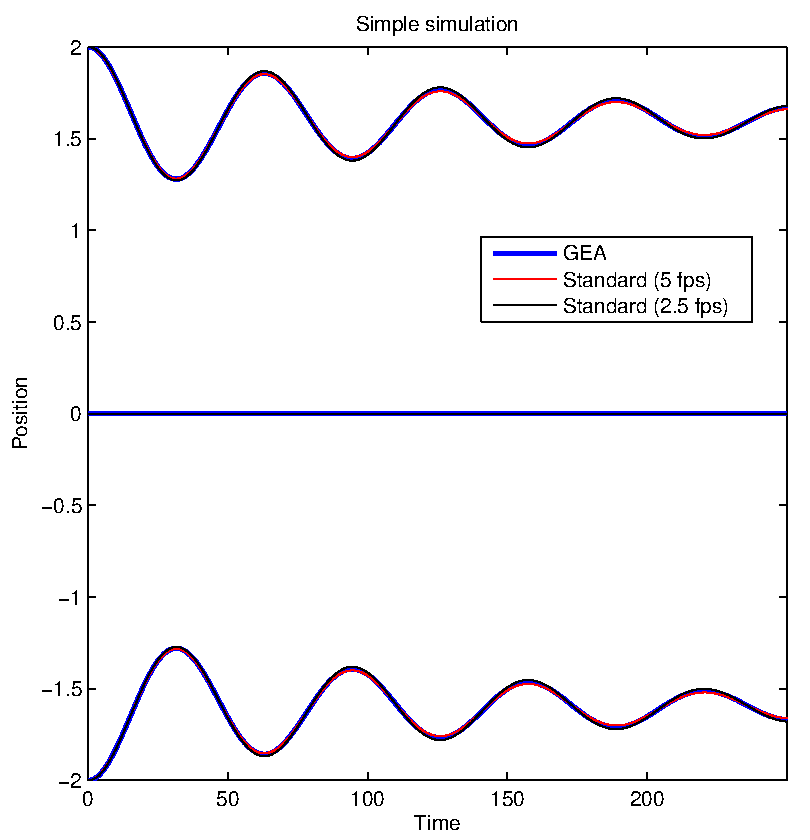
\includegraphics[width=\textwidth]{../images/inverse_uniform_30fps.pdf}
        \caption{Simulation using GEA (blue) and standard (red) simulation methods with
        position as a function of the time of the simulation.}
        \label{fig:inverse_uniform_30fps_0}
    \end{subfigure}
    \begin{subfigure}[t]{0.5\textwidth}
        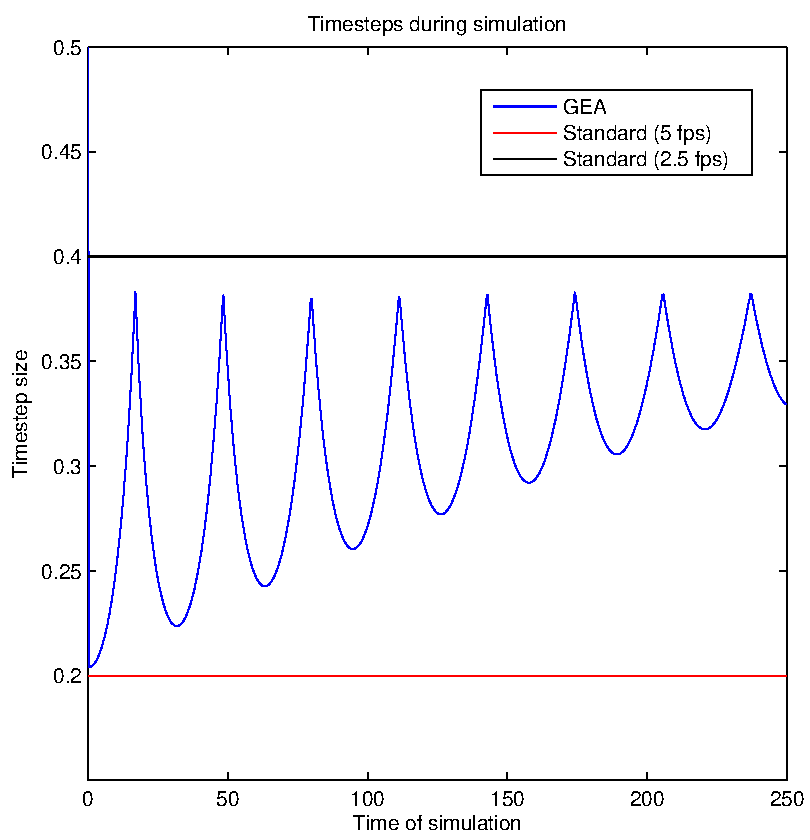
\includegraphics[width=\textwidth]{../images/inverse_uniform_30fps_steps.pdf}
        \caption{Timestep size for GEA (blue) and standard (red) of the simulation in
            \ref{fig:inverse_uniform_30fps_0}}
        \label{fig:inverse_uniform_30fps_steps}
    \end{subfigure}
    \caption{GEA compared with standard simulation on simple 3-vertex
    mass-spring system}
    \label{fig:inverse}
\end{figure}
\begin{figure}
    \begin{subfigure}[t]{0.5\textwidth}
        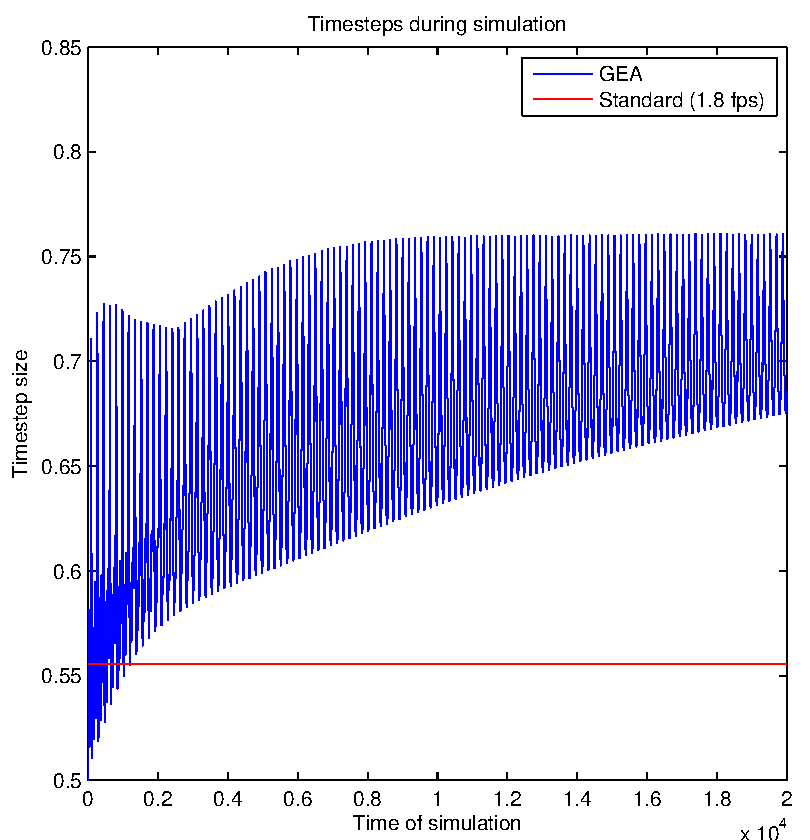
\includegraphics[width=\textwidth]{../images/inverse_multiscale_steps.pdf}
        \caption{Timestep size for GEA (blue) and standard (red) as a function
        of the time passed}
        \label{fig:inverse_multiscale_steps}
    \end{subfigure}
    \begin{subfigure}[t]{0.5\textwidth}
        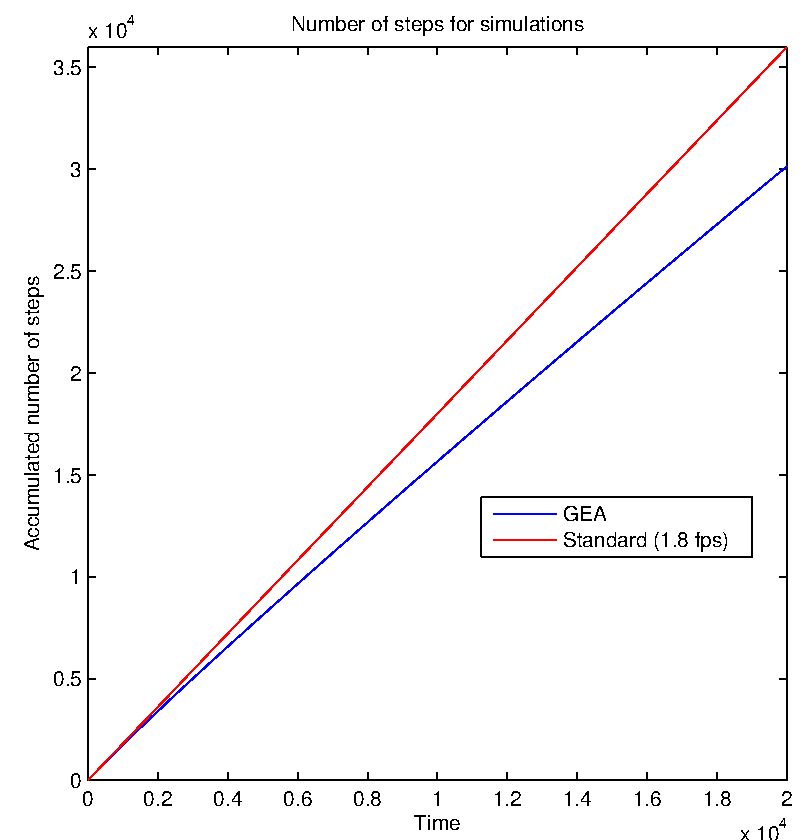
\includegraphics[width=\textwidth]{../images/inverse_multiscale_cumstep.pdf}
        \caption{Accumulated number of steps taken as a function of the time passed for GEA
        (blue) and standard (red)}
        \label{fig:inverse_multiscale_cumstep}
    \end{subfigure}
    \caption{GEA compared with standard simulation on particles distributed with
        two scales simulated for 20,000 seconds}
    \label{fig:inverse_multiscale}
\end{figure}

%Examples of
%
%\begin{table}[H]
%\caption{Example table}
%\centering
%\begin{tabular}{llr}
%\toprule
%\multicolumn{2}{c}{Name} \\
%\cmidrule(r){1-2}
%First name & Last Name & Grade \\
%\midrule
%John & Doe & $7.5$ \\
%Richard & Miles & $2$ \\
%\bottomrule
%\end{tabular}
%\end{table}

%------------------------------------------------

\section{Future work}

Combine atomic approach with inverse acceleration heuristic

Test methods with other integration schemes

Test methods with hyperelastic materials

Relate to hyperelastic materials (some linear heuristic = win)

%------------------------------------------------

\section{Conclusion}


%----------------------------------------------------------------------------------------
%	REFERENCE LIST
%----------------------------------------------------------------------------------------


\bibliography{bibliography}
\bibliographystyle{plain}

%----------------------------------------------------------------------------------------


\end{document}
